%%% Fiktivní kapitola s ukázkami sazby

\chapter{Návrh}

Kapitola návrh se věnuje dvou tématům. V první části se věnuje návrhu uživatelského rozhraní a přechodů mezi obrazovkami. V druhé části se věnuje tradičnějšímu chápání slova návrh ve vývoji, a to softwarové architektuře. Cílem návrhu je vytvořit 

\section{Uživatelské rozhraní}

Návrh uživatelského rozhraní je disciplínou softwarového inženýrství, která se věnuje návrhu uživatelského rozhraní na koncepční úrovni. Při vytváření uživatelského rozhraní je nutno brát v potaz požadavky uživatelů, aby nebylo ubíráno na efektivitě aktivity uživatele v aplikaci. Cílem je navrhnout uživatelské rozhraní pro uživatele rychlo uchopitelné a přehledné. V disciplíně návrhu uživatelského rozhraní se využívá mnoho modelovacích technik, např. prototypování a drátěné modely. Pro správné posouzení efektivnosti uživatelského rozhraní je nutno tyto modely konfrontovat s potenciálními uživateli a sledovat jejich reakce a přpomínky a reflektovat je v následujících iteracích návrhu uživatelského rozhraní. 

Pro tuto práci byla zvolena technika drátěných modelů (tzv. wireframe), schematickým nákresem prvků na obrazovce a jakým způsobem do sebe zapadají (ref). Tyto návrhy jsou ušetřeny komentářů, které součástí wireframů někdy bývají. V rámci této práce nebylo možno provádět studie mezi potenciálními uživateli, byl zvolen alternativní způsob inspirace známými UI elementy, které jsou přítomny v jiných aplikacích. 

% https://www.academia.edu/6511543/The_Elements_of_User_Experience_User-Centered_Design_for_the_Web_and_Beyond_Second_Edition p. 128

\subsection{Onboarding, přihlášení, registrace}

\begin{figure}[h]
	\begin{center}
		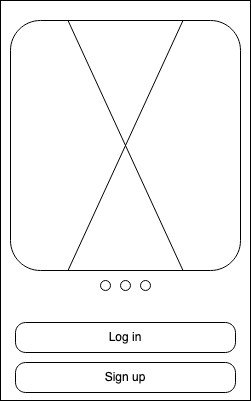
\includegraphics[width=70mm]{img/wf_onboarding.png}
		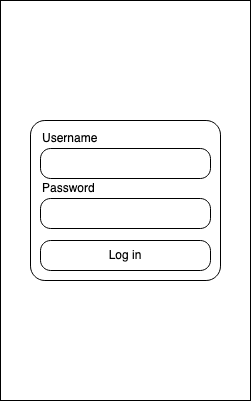
\includegraphics[width=70mm]{img/wf_login.png}
	\end{center}
	\caption[Wireframe přihlášení a onboarding obrazovky]{Wireframe onboarding a přihlašovací obrazovky -- zdroj: autor}
	\label{fig:boat1}
\end{figure}

Pro přihlašovací obrazovku byl zvolen koncept tzv. onboardingu, praktiky popisující funkce aplikace a výhody založení účtu. Onboarding lze také chápat jako náhradu aplikačního návodu. Onboarding může být prováděn mnoha způsoby, jako nejsnadněji řešitelný byl vybrán tzv. carousel, seznam posouvatelných panelů, kde každý z nich obsahuje určité informace o mobilní aplikaci. Pro přihlašovací obrazku byl zvolen očekávatelný klasický formát přihlašovacího dialogu. Pro registraci byl využit tzv. web view, komponenta, co zobrazí webový prohlížeč svázaný s aplikací. Registrace se tedy provádí přes stávající webovou aplikaci. Důvodem tohoto rozhodnutí je absence API pro vytváření uživatelských účtu, ale zároveň i předpoklad, že uživatel mobilní aplikace bude i zároveň uživatelem aplikace webové.

\subsection{Mapová koncepce}

Hlavní obrazovkou aplikace byla zvolena obrazovka s mapou, aby odpovídala očekávání uživatelů webové aplikace Anitra, kde hlavní obrazovkou je taktéž mapa. Veškeré kontrolky, které by se daly zobrazit jako separátní stránky, se zobrazují v modálních oknech nad obrazovkou, což je opět koncepce vycházející z již hotové webové aplikace. Aplikace tedy rovnou splní jeden ze zmíněných případů užití při zapnutí, a to kontrolu posledních pozic trackerů a případné odfiltrování pro uživatele nezajímavých trackerů způsoben srovnatelným s aktuálním řešením, čímž by se dalo očekávat zkrácení doby učení uživatelů aplikace.

\section{Aplikační architektura}

%Clements, Paul; Felix Bachmann; Len Bass; David Garlan; James Ivers; Reed Little; Paulo Merson; Robert Nord; Judith Stafford (2010). Documenting Software Architectures: Views and Beyond, Second Edition. Boston: Addison-Wesley. ISBN 978-0-321-55268-6.

Aplikační (resp. softwarová) architektura popisuje strukturu softwarového systému. Struktura softwarového systému obsdahuje softwarové elementy, jejich vztahy a vlastnosti elementů a jejich vlastností (ref). Přístupy k této disciplíně se liší dle metodiky vývoje softwaru, rigozórní metody preferují architekturu dopředu pevně formulovat, zatímco více agilní metodiky pravý opak. V rámci této práce softwarová architektura nebyla řešena příliš do podrobna, jelikož se jedná o velmi malou aplikaci.

\subsection{Základní koncepce}

Pro řešení aplikace byly zvoleny architektonické vzory, tedy typické architektury, které se v návrhu softwarových architektur často vyskytují. Aplikace byla navrhnutá jako dvouvrstvá klient-server aplikace, kde první vrstva zajišťuje operaci s daty (modelová vrstva, podkapitola Datové zdroje a entity) a druhá vrstva správné zobrazení (prezentační vrstva, podkapitola Komponenty). Tento koncept byl zvolen díky plnému splnění architektonických nároků malé aplikace a komponentové architektuře React.

\subsection{Datové zdroje a entity}

\subsection{Komponenty}

